\subsection{Forberedelse av lydfil for analyse}
For å kunne ta i bruk den numeriske løsningen av bølgeligningen, må lydfilen først forberedes. Dette gjøres ved å lese inn lydfilen 
og konvertere den til et format som kan brukes i den numeriske modellen. I dette prosjektet benyttes Python-biblioteket 
\verb|scipy.io.wavfile| for å lese inn lydfilene i WAV-format. Det er blitt valgt å bruke en avgrenset del av lydfilen for å redusere kompleksiteten
i analysen og fokusere på de mest relevante delene av signalet. Dette lar oss også identifisere enkelte toner med STFT-analyse og forhåpentligvis kunne
identifisere instrumentene som produserer disse tonene.

Når det gjelder samplingsrate, ble det brukt den standard samplingsraten på 44100 Hz for lydfilen. Dette er en vanlig samplingsrate for 
lydfiler og gir en god balanse mellom lydkvalitet og filstørrelse. Dette gir en analyserekkevidde opp til 22050 Hz, i henhold til Nyquist-teoremet.
Det også viktig å velge en høy nok samplingsrate for å sikre at de høyeste frekvensene i lydsignalet blir korrekt representert, hvis ikke kan aliasing oppstå.

\subsection{Analyseringsprogram i python}

I dette delkapittelet beskrives koden for å fouriertransformere en sangfil, med fft. Koden kan hentes her: 
\parencite{python_fft_analyse} 

For å analysere lydsignalet til en sang, har programmeringsspråket python blitt brukt, da med
pakkene \texttt{numpy}, \texttt{matplotlib}, og \texttt{scipy}for å animere og plotte grafen. 
Pakkene \texttt{subprocess}, \texttt{progressbar}, og \texttt{argparse} har blitt brukt for 
å kjøre eksterne programmer, se status på rendering av animasjon og hente inn kommandolinjeargumenter når
programmet blir kjørt. 

\subsubsection{Animasjonsfunksjonen}

Først brukes \texttt{scipy} biblioteket sin funksjon \texttt{wavfile.read} for å lese av input filen.
Denne returnerer \texttt{sampleRate}, som er hvor mange ganger per sekund den analoge bølgen for 
sangen har blitt målt. Det andre funksjonen returnerer er \texttt{wav}, som er array fra 
\texttt{numpy} biblioteket. Denne arrayen består av alle samplingene til sangen. Deretter blir
lengden på arrayen lest av for å finne ut hvor mange samplinger det er i sangen. 

Ettersom samples i en wav fil kan bli enten lagret som \texttt{float} (desimaltall) fra 
\texttt{[-1.0 , 1.0]} eller \texttt{int16} (16 bit integer) fra \texttt{[-32768 , 32768]}, brukes det
en \texttt{if}-sjekk for å sørge for at det kun er desimaltall innenfor \texttt{[-32768 , 32768]} 
som brukes for å tegne på grafen. Deretter blir wav-arrayen sjekket for om det er en eller 
to kanaler. Dersom det er to kanaler, blir kanalene lagt sammen til en kanal for å få med seg
alle frekvensene uten å måtte fouriertransformere hver kanal for seg. 

Deretter kommer seksjonen i koden der viktige variabler blir satt. Først defineres \texttt{spf} eller \textit{samples per frame}, 
, som er antall samplinger mer bilde som renderes i animasjonen. Deretter defineres \texttt{T = 1.0 / sampleRate}, som er 
hvor lang tid det er mellom hver sample i wav-filen. Antall samples per fouriertransformasjon defineres av 
\texttt{N = max(2, fftTime * sampleRate)}, der \texttt{fftTime} er ett av funksjonsargumentene, som definerer
hvor langt tidsintervall som skal fouriertransformeres om gangen. For å finne ut hvor mange bilder som skal lages
i videoen, brukes formelen  \texttt{totalFrames = max(o , (len(wav) - N) // spf + 1)}. Stykket finner ut hvor mange samples 
som er med, minus ett vindu, og deretter delt på antall samplinger per bilde. 

For å regne ut hvilke verdier en for langs x-aksen, blir \text{scipy} biblioteket sin \texttt{rfftfreq} funksjon brukt.
\texttt{rfftfreq(N, T)} returnerer en array av positive frekvensverdier, frem til Nyquist-frekvensen som er halvparten
av samplingsraten. \texttt{[: N //2]} gjør at frekvensaksen passer med resultatet for fouriertransformasjon av signalet.

\subsubsection{Fouriertransformasjon per bilde}

Det er funksjonen \texttt{fftWav(n)} som håndterer fouriertransformasjon per bilde i animasjonen. Variablen \texttt{n}
representerer bildenummeret i hele arrayen. Funksjonen starter ved å definere \texttt{n0} og \texttt{n1}, som er rammene
til hvor i wav-arrayen en skal fouriertransformere fra og til. Dette skjer ved å definere \texttt{fftwav = wav[n0:n1]}, 
som kutter \texttt{wav} fra \texttt{n0} til \texttt{n1}. \texttt{n0} blir bestemt ved uttrykket \texttt{n * spf - N // 2},
der den hopper \texttt{n * spf} samplinger frem i wav-arrayen, og trekker fra halvparten av \texttt{N} som startverdi.
Deretter sjekkes det om arrayen som skal fouriertransformeres for bildet er like lang som \texttt{N}. Hvis ikke legges
det til ekstra verdier for å få arrayen til riktig størrelse. Dette betyr at de siste bildene vil ha noe unøyaktig 
fouriertransformasjon. Denne arrayen blir så multiplisert med hanning-vinduet \texttt{window}. Deretter fouriertransformeres arrayen \texttt{fftWav} med \texttt{scipy} sin funksjon \texttt{rfft}.
Den nye arrayen blir kalt \texttt{yf}. Nå kan denne arrayen inneholde negative verdier, derfor må en gjøre disse positive og 
normalisere resultatet. 

\begin{figure}[H]
	\centering
	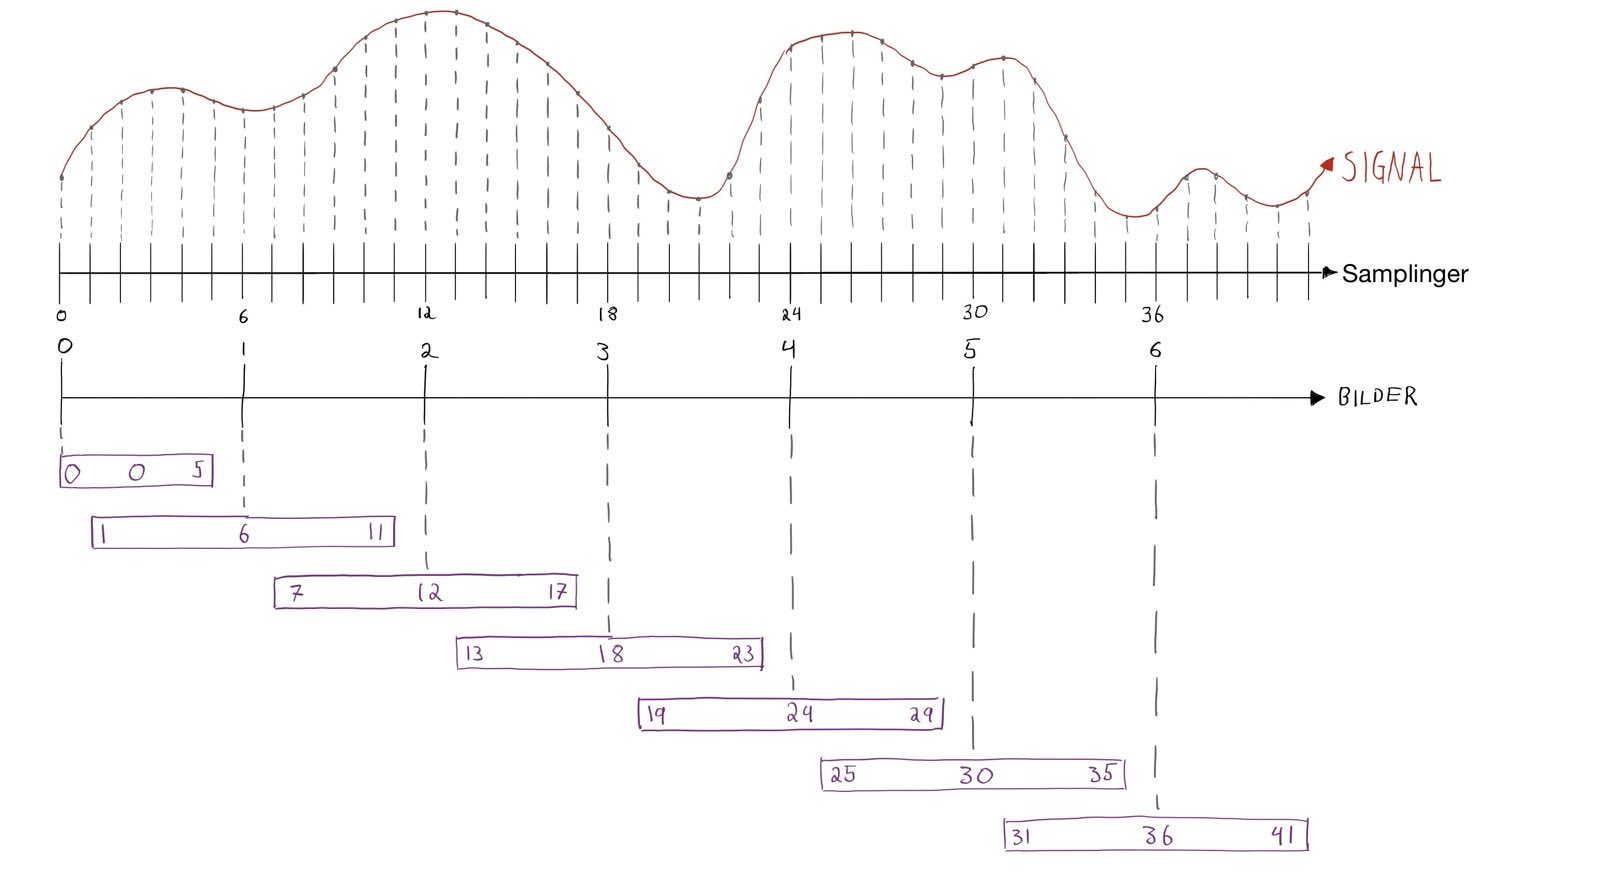
\includegraphics[width=\textwidth]{figurer/samplinger-og-bilder-sammenheng.jpg}
	\caption{Sammenheng mellom sampling og bilder eksempel}
	\label{fig:eksempelSammenhengSamplingOgBilder}
\end{figure}

Figur (\ref{fig:eksempelSammenhengSamplingOgBilder}) viser sammenhengen mellom hvordan programmet håndterer ulike 
fouriertransformasjonsvinduer og ulike bildefrekvenser. Fra eksempelet er det plottet \texttt{41} ulike samplinger, med
en samplingsrate på \texttt{sampleRate = r = 100Hz}. Bildefrekvensen er satt lik \texttt{fps = 16}. Dette gir en samplinger per bilde
verdi på \texttt{spf = 100 / 16 = 6}. Det er satt en tidsluke for hver fouriertransformasjon til \texttt{fft\_t = 0.1s}. Det gir 
antall samplinger per fouriertransformasjon \texttt{N = r * fft\_t = 100Hz * 0.1s = 10}. Betydningen av det
er at for hver sjette sample, renderes det ett nytt bilde. Bildet tar for seg \texttt{N} antall samplinger i fouriertransformasjonen
for bildet. For å få mest mulig overlapp mellom bilder, er blir tar den med fem samplinger før og etter bildet sin
"senter" sampling, som er bestemt av \texttt{n * spf}.

\subsubsection{Plotting og animasjon av bilder}

Ettersom at de høyeste og laveste amplitudeverdiene på ulike lydfiler kan være svært ulik hverandre, starter koden
for plotting ved å finne en maksverdi for amplitude. Det skjer i form av en for-løkke som itererer fra null til 
totale bilder i samplearrayen. Der den for hver iterasjon gjør fouriertransformasjonen, og via funksjonen 
\texttt{np.percentile} finner den gjennomsnittet av $99\%$ av verdiene i den fouriertransformerte arrayen.

Deretter defineres plottingargumentene. Her er navngis aksene, og maksverdi for x og y aksen defineres her. 
Deretter kommer \texttt{animate} funksjonen. Funksjonen tar bildenummer \texttt{i} som argument, og returnerer
\texttt{xf} som x-akse verdier og den fouriertransformerte fo bildet \texttt{y} som grafen. I tilleg blir 
\texttt{infoTekst} returnert, som er boksen i høyre hjørne som viser ulike parametre for hvert bilde. For animasjon
blir funksjonen \texttt{FuncAnimation} brukt. Den tar plottingfigur \texttt{fig}, animasjonsfunksjon \texttt{animate},
initialiseringsfunksjon \texttt{init}, antall bilder \texttt{totalFrames}, tidsintervall mellom hvert bilde 
\texttt{1000/ fps}. For å lagre plotten, brukes funksjonen \texttt{anim.save} brukt. Den lagrer videoen i en 
midlertidig fil, der \texttt{subprocess} biblioteket sin funksjon {sp.run} blir brukt til å kjøre 
\texttt{ffmpeg} programmet for å legge til lyd på programmet. 

\subsection{Spektrogramanalyse i Python}

I dette delkapittelet beskrives koden som brukes for å analysere lydsignalet til sangen 
\textit{Seven Nation Army}, ved å beregne og visualisere et melspektrogram. Programmet 
er skrevet i Python, og benytter pakkene \texttt{librosa}, \texttt{numpy} og \texttt{matplotlib} 
for å lese, behandle og plotte lyddataen. Koden kan hentes her: \parencite{python_mel_spektrogram}

\subsubsection{Melspektrogramfunksjonen}

Først lastes lydfilen inn ved hjelp av funksjonen \texttt{librosa.load}. Denne returnerer 
to verdier: \texttt{y}, som er selve lydsignalet som et array av amplitudeverdier, og 
\texttt{sr}, som er samplingsfrekvensen. Samplingsfrekvensen angir hvor mange ganger per sekund 
den analoge lydbølgen har blitt målt:

\begin{equation*}
    \Delta t = \frac{1}{sr}
\end{equation*}

Signalet \texttt{y} kan dermed beskrives som en tidsdiskret sekvens:

\begin{equation*}
    y = \{x[n]\}_{n=0}^{N-1}
\end{equation*}

hvor \( x[n] \) representerer lydens amplitude ved tidspunkt \( t = n \cdot \Delta t \).

Deretter beregnes et melspektrogram ved hjelp av funksjonen \texttt{librosa.feature.melspectrogram}. 
Denne funksjonen utfører en korttids Fourier-transformasjon (STFT) av signalet:

\begin{equation*}
    X(k,m) = \sum_{n=0}^{N-1} x[n+mH]\, w[n]\, e^{-j2\pi kn/N}
\end{equation*}

Her er \( w[n] \) vindusfunksjonen, \( H \) hop size (forskyvning mellom vinduer), 
\( k \) frekvensbånd og \( m \) tidsvindu.

Etter at STFT er beregnet, konverteres frekvensaksen fra lineær skala til mel-skala, 
som er tilpasset hvordan mennesket oppfatter tonehøyde. Denne skalaen defineres ved:

\begin{equation*}
    \text{mel}(f) = 2595 \cdot \log_{10}\left(1 + \frac{f}{700}\right)
\end{equation*}

Energien i hvert frekvensbånd summeres innenfor et gitt antall mel-bånd for å representere 
lydens spektrale energi på en perceptuell skala.

Videre konverteres energiverdiene i spektrogrammet til desibel (dB) for å fremheve variasjoner 
i lydstyrke. Dette gjøres med:

\begin{equation*}
    S_{\text{dB}} = 10 \cdot \log_{10}\left(\frac{S}{S_{\text{ref}}}\right)
\end{equation*}

hvor \( S_{\text{ref}} = \max(S) \) brukes som referanseverdi slik at den sterkeste 
frekvenskomponenten blir 0 dB.

Til slutt visualiseres melspektrogrammet ved hjelp av funksjonen \texttt{librosa.display.specshow}, 
der x-aksen representerer tid, y-aksen mel-frekvens, og fargene intensitet i dB. Et fargekart viser variasjonen i energi over tid og frekvens, der lysere farger indikerer høyere energi. Figuren viser hvordan frekvensinnholdet i sangen endrer seg over tid, og gir et visuelt grunnlag for videre analyse av rytme og struktur.




